\section{Panorama} \label{sec:panorama}
%在我们深入讲解我们的系统之前,我们首先给出一个我们整个系统的全景图,如图1所示。这张全景图在一张图内尽可能详细的描述了我们尝试解决可什么问题以及如何解决了这个问题。

Before digging into the details of HyperPS, we first give a panorama view of our system, as depicted in Figure \ref{pic:panorama}. This figure sketches in detail what problem we tried to solve and how we solve it.
In this section, we first elaborate on our motivation to protect VMs under a compromised HostOS/Hypervisor. Then, we explain some necessary background for a better understanding to Figure \ref{pic:panorama} and HyperPS. Finally, we present our threat model.

%要在标题上对整个系统进行简单说明,既然是全景图,那么就应该包括如下的几点:要干什么,这个要最开始说,就一句话,说明我们要干什么,在这里就是如何在Hypervisor已经被危害的情况下如何保护guestVM的安全。这样就不需要说明威胁模型了,因为上面已经说了,是在Hypervisor已经被危害的前提下,就概括了图左边的内容;简要说明架构,这里要突出两个东西,一个是同层隔离,一个是将VMCS EPT移除到新的空间中。这个也是本文的两个最主要的东西,前者同层隔离提一句,要不要说好处呢?用修饰词把。后面VMCS,写效果,即VMCS移除以后会有什么效果,这个也是我们的最终的目的。
%HperPS利用内核页表构造一个与HostOS Hypervisor具有相同特权级的空间,并剥夺了原有内核对VMCS EPT的管理的特权,并将对应的特权赋予在隔离空间的Secure Code。
%HyperPS致力于在VMM HostOS已经被Compromised的前提下,剥离VMM直接管理VM的相关功能(VMM最重要的目的就是管理VM,现在将其最重要的功能剥离了,那么还要这个东西干啥用?)实现对保护VM的安全。
%TODO 修改,将HyperPS的Isolated 修改为separated
\begin{figure*}
    \centering
    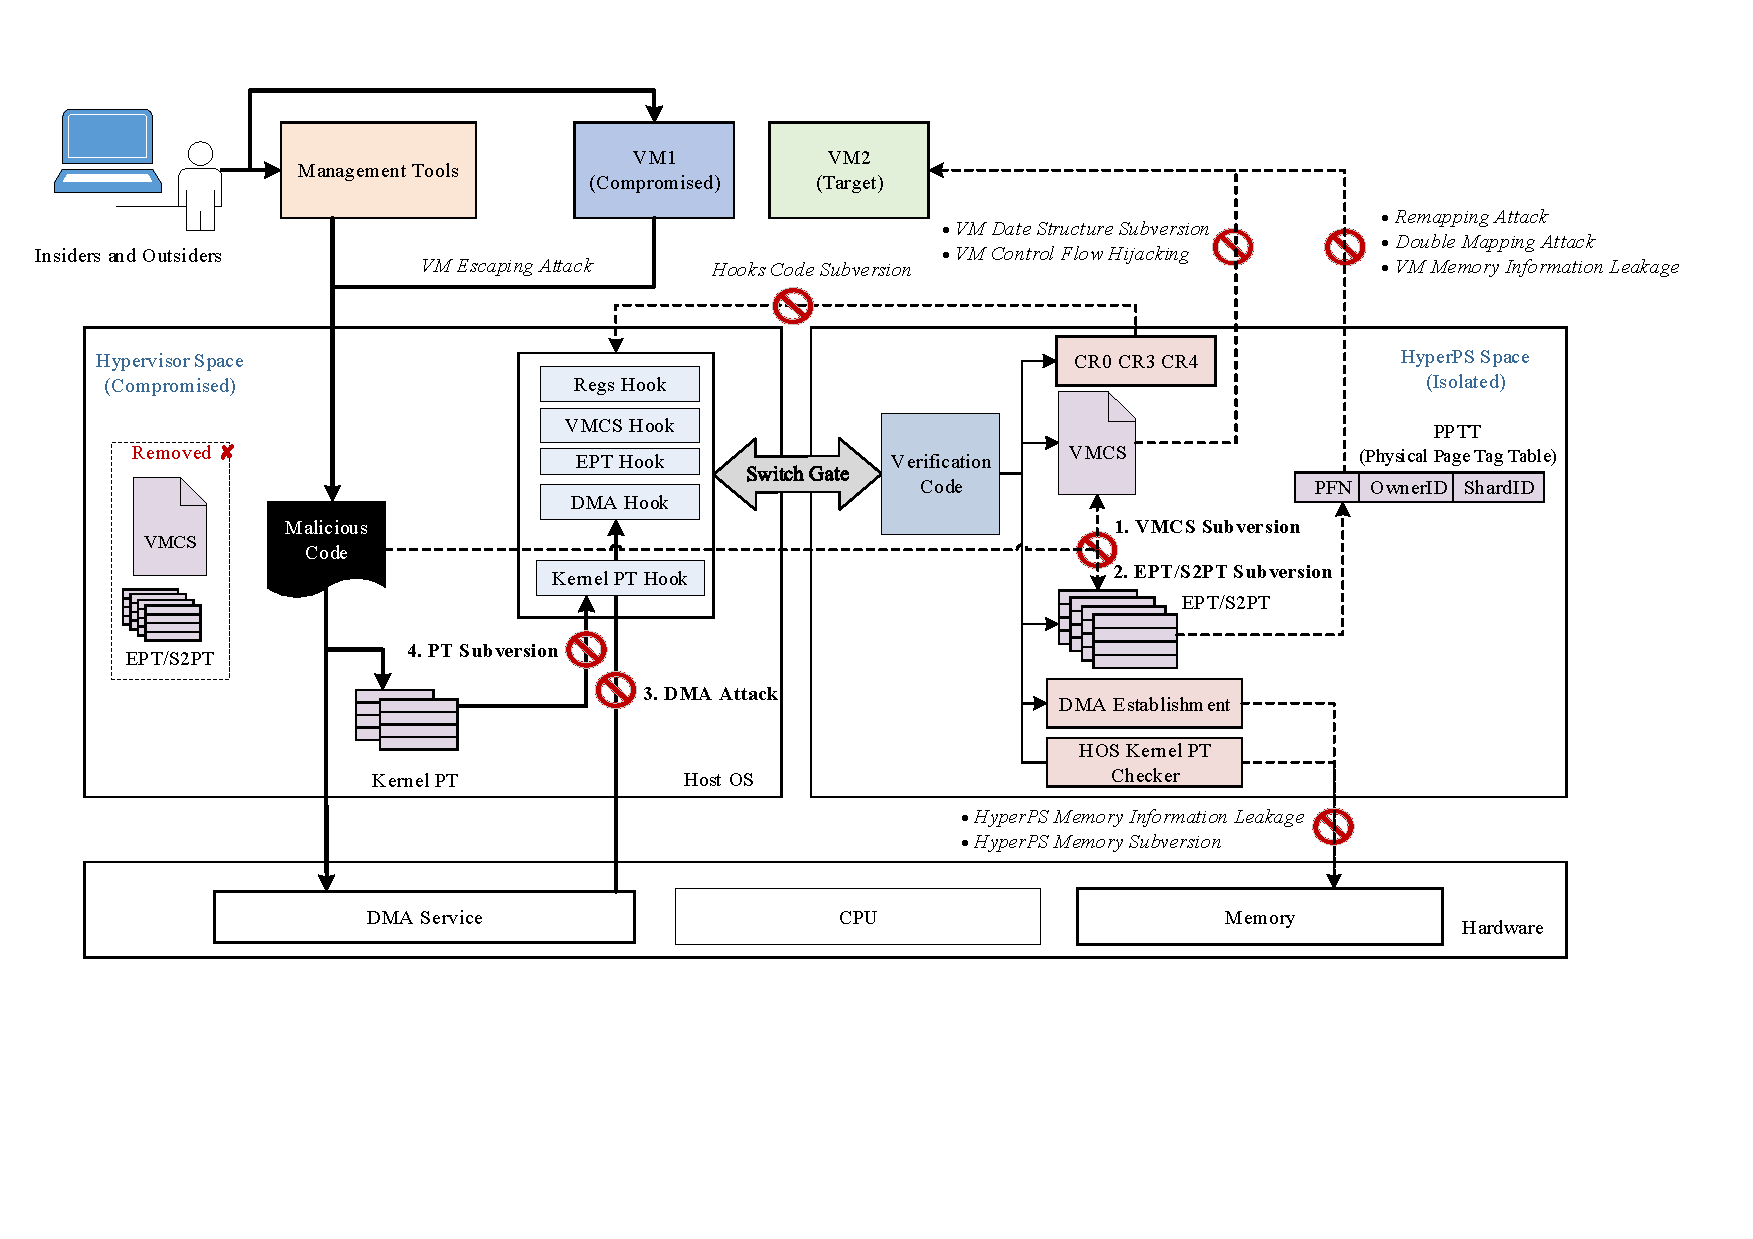
\includegraphics[width=1\textwidth]{IMG/panorama.pdf}
    \caption{The Panorama View of HyperPS. \\ HyperPS is committed to protect guest virtual machine under the compromised HostOS/Hypervisor. Privileges to manage VMCS and EPT are stripped from the compromised HostOS/Hypervisor into a separated and secure execution environment: HyperPS Space. The HyperPS space shares the same processor privilege as the HostOS. HyperPS does not rely on any special hardware or a higher privilege. Updates to VMCS and EPT are abandoned by the HyperPS, if the operations are not authorized or are adjudged as harmful to virtual machine.}
    \label{pic:panorama}
\end{figure*}

\subsection{Motivation} \label{sub:motivation}

\iffalse
#######################
###### 写作分析 ####### 
#######################
我们为什么要提出这个观点?首先明白一点:我们是站在VM角度上来思考问题的吗?假如VM不信任下面的VMM,那么就不应该上云,任何安全都不能保证。那么VM租户的角度是否能要求下面提供一个更加安全的架构,应该,但是不应该是租户要求下面的云服务提供商来采用我们的架构,因为一旦是要上云了,人家提供了什么你就选择什么,不能要求其更改云的架构。所以,站的视角一定不是VM租户的角度。那么角度就应该是下面的VMM。就是云服务提供商。对于VMM,其有什么动力要更改他们现在的架构?而不是现在的架构,毕竟无论如何一个同层隔离也更改了现有的云架构了。所以这里不应该假定存在内部攻击者,内部工作人员本身就知道我们的架构的存在,完全可以卸载了就好了,不需要还进行什么防护。所以,只可能存在一种情况,就是云服务提供商也不能完全保证其hostos的安全,但是其最核心的功能应该是如何保证其云的功能是安全的。所以,采用同层隔离的功能将云的相关功能隔离起来。从而实现云部分的安全。换句话说,就是,即使在HostOS存在脆弱点,其已经被攻击者攻陷的前提下,或者上面的VM通过虚拟机逃逸已经获取了下面的os的部分权限的前提下,如何保证VM的安全,即仍然能提供正常的云服务,保证用户的安全。那么前提就是云服务提供商也不完全信任下面的hostOS内核。
这段内容是否是我们的motivation?是,要详细写出来,但是思路不应该说VM租户内容,而应该从后面的内容出发,这个内容要不要在instruction中写出?要,但是要简洁,这里是详细说明。

基于上面的分析,我们假定的威胁模型应该是攻击者可以利用内核的脆弱性,获取了部分hostOS的权限,这权限是什么?这个要详细说明。
首先是最常见的,任意内存读写权限?或者特定的内存的读写权限?能否嵌入shellcode?这些要详细的分析,但是这个部分的工作放到后面,先将motivation写出来。

因为下面的Linux其实有很多脆弱点的,但是在传统的qemu-kvm的框架中,任何
这里首先要讲出如果HostOS并不安全,
The motivation for this work derives directly from
这部分要写出我们为什么要做这个系统,初衷是什么,要解决什么问题。

这部分要写什么?怎么写?
要按照这个逻辑来写:首先最开始用几句话说明云服务提供商最重要的任务是保证上面组会的安全,这是其需要负责的责任。然后需要论证hostos是不安全的,在这个条件下,其云系统可能被危害,一旦HOSTOS被危害,那么就无法保证上面VM的安全,立脚点一定是站在云服务提供商的角度上。最后自然而然的引出我们的motivation,就是如何在hostos被危害的前提条件下,云服务提供商如何保证虚拟机的安全。
\fi

\iffalse
##############################
##### Motivation中文初稿 #####
##############################
云服务商需要向云租户提供的众多服务中,能保证虚拟机的完整性和安全性是是其获取用户信任的关键因素。
对于每一台虚拟机,云服务提供商需要保证用户虚拟机的运行不会被侵害,其运算不会被恶意篡改,其数据不会被盗取。对于同属一个平台的不同服务器之间,云服务提供商需要保证不同虚拟机之间的有效隔离。但是,在QEMU-KVM架构中,作为HostOS的Linux不仅仅是一个负责提供虚拟化服务的hypervisor,还是一个正常的操作系统。
% HostOS在除了负责虚拟化相关核心功能之外,还是一个
即使云服务商采用定制的精简的Linux作为hostos,其仍然含有大量的与虚拟化功能无关的各种子系统subsystem,而这些功能,特别是来源复杂的内核驱动等不可避免的含有大量的可以被利用的内核脆弱点。这就提供给了攻击者一个巨大的攻击面surface,即使攻击者没有找到可以利用的QEMU/KVM脆弱点,其仍然可以通过exploit Linux其他subsystem的脆弱点实现对虚拟化部分的危害。云服务提供商并不能有效的保证Linux subsystem 特别是大量驱动设备的安全性,因此,云服务提供商需要进一步思考如何在hostos已经被危害的前提下保证虚拟机的安全,这就是HyperPS的motivation。
\fi

In this section, we discuss the motivations of why we need to protect VMs under an untrusted HostOS/Hypervisor.

Among the many services that cloud service providers need to provide to cloud tenants, ensuring the integrity and security of virtual machines is the key factor in gaining user trust. For each VM, the cloud service provider needs to ensure that the user's business in the VM will not be maliciously tampered with, and the data will not be stolen. For different VMs, cloud service providers need to ensure effective isolation between different VMs. However, in the QEMU-KVM architecture, Linux as HostOS is not only a hypervisor that is responsible for providing virtualization services, but also a normal operating system with full functions. In a real business deployment, even if cloud service providers adopt customized Linux as the HostOS, the Linux kernel still contains a large number of various subsystems that have nothing to do with virtualization. These subsystems, especially kernel drivers with complex sources, inevitably contain countless exploitable vulnerabilities. These subsystems provide the attacker with a huge attack surface. Even if the attacker does not find any exploitable QEMU or KVM vulnerabilities, he can still tamper with the virtualization component by exploiting the vulnerabilities of other Linux subsystems. Therefore, cloud service providers need a further think about how to ensure the security of VMs under the premise that the HostOS/Hypervisor has been compromised. This is the motivation of our HyperPS.


\subsection{Background}%
\label{sub:background}
This section presents some necessary background knowledge to facilitate readers to better understand HyperPS and threat model depicted in Figure \ref{pic:panorama}.
\subsubsection{QEMU-KVM}%
\label{ssub:qemu_kvm}
QEMU is a generic and open source machine emulator and virtualizer. QEMU can use other hypervisor like \verb|Xen| or KVM to use CPU extensions for virtualization. When used as a virtualizer, QEMU achieves near native performances by executing the guest code directly on the host CPU.
Kernel-based Virtual Machine (KVM) is an open source virtualization technology that converts Linux into a type-1 (bare-metal) hypervisor. KVM is a part of the Linux kernel that shares all the linux kernel's operating system-level components -such as the memory manager, process scheduler, security manager, and more to run VMs. Every VM is implemented as a regular Linux process, scheduled by the standard Linux scheduler, with dedicated virtual hardware like a network card, memory, and disks. KVM mainly consists of a loadable kernel module, kvm.ko, that provides the core virtualization infrastructure and a processor specific module, kvm-intel.ko or kvm-amd.ko.
In virtualization environment, KVM does not work on its own. It is only an API provided by the kernel for userspace. End users typically use KVM through QEMU where it is present as an acceleration method.
For the QEMU-KVM architecture, KVM interacts with QEMU (QEMU runs at the user space) in two ways: through device file \verb|/dev/kvm| and through memory mapped pages
% KVM interacts with user space - in most case QEMU - in two ways: through device file \verb|/dev/kvm| and through memory mapped pages.
Memory mapped pages are used for bulk transfer of data between QEMU and KVM. \verb|/dev/kvm| is the main API exposed by KVM. It supports a set of \verb|ioctl|s which allow QEMU to manage VMs and interact with them.
% 怎么引出HostOS的问题
% Since KVM is a part of the linux kernel, the Linux and the QEMU
% leverages the linux kernel's system-level



\subsubsection{VMCS}%
\label{ssub:vmcs}
Virtual-machine Control Structure is a data structure used in Virtual Machine eXtensions (VMX). It controls VMX non-root operations (guest virtual machine execution operations) and VMX transitions. Access to the VMCS is managed through the VMCS pointer (one per logical processor). The VMCS pointer is read and written suing the instructions \verb|VMPTRST| and \verb|VMPTRLD|. In general, the hypervisor configures a VMCS using \verb|VMREAD|, \verb|VMWRITE|, and \verb|VMCLEAR| instructions. A hypervisor could use a different VMCS for each virtual machine that it supports. For a virtual machine with multiple logical processor, the hypervisor could use a different for each logical processor. A logical processor may also maintain a number of VMCSs that are active, however, at any given time, at most one of the active VMCSs is the \textbf{current} VMCS. VMX instructions operate only on the \textbf{current} VMCS. 

%这段写的不好,没有写出危害的具体内容,应该突出VMCS就是唯一的接口,VM的所有的行为都是在VMCS的instruct下的
A compromised HostOS/hypervisor can force the guest virtual machine exit by tramper VM-Execution Control fields and VM-exit control fields in VMCS and tramper the guest virtual machine by writing Guest-State Area fields. 

% 一个被危害的hypervisor可以强迫虚拟机退出,并通过篡改其vmcs中的field等信息实现对guest VM 的危害。

% \subsection{Second Level Address Translation}%
% \label{sub:second_level_address_translation}
% Second Level Address Translation (SLAT) is a hardware-assisted virtualization technology which makes it possible to quick manage the physical memory without lots of VM exits. Extended Page Table (EPT) is the intel's implementation of SLAT, while ARM names its implementation as Stage-2 Page-tables.


\subsubsection{EPT}%
\label{ssub:ept}
Intel implements it Second Level Address Translation (SLAT) as Extended Page Table (EPT). 
EPT allows each virtual machine to manage its page table (not the EPT), without giving access to the underlying host machine's MMU Hardware. Thus, EPT reduces the need for hypervisor to keep syncing the shadow pages eliminating the overhead.
If EPT is enabled, guest-physical addresses are translated by traversing a set of EPT paging structures to produce physical addresses that are used to access memory.
In addition to translating a guest-physical address to a physical address, EPT specifies the privileges that software is allowed when accessing the address. Attempts at disallowed accesses are called EPT violations and cause VM exits.

A compromised HostOS/hypervisor could tramper EPT paging structures so that the virtual machine will execute arbitrary malicious code without knowing it. 
Moreover, a compromised HostOS/Hypervisor could access any data in the guest virtual machine with the help of virtual machine introspection.



%\subsection{Attacks and Threat Model} \label{sub:thretmodel}
\subsection{Attack Surface}\label{sub:attacksurface}
\iffalse
在这一章节中,我们首先给出攻击者的攻击路径,这个攻击路径并不需要单独画图,因为上面的图中已经阐释清楚了,攻击者有哪些方式可以危害虚拟机,只需要在图中更加明确的标识出来就可以了。然后再给出本文的威胁模型。

首先一句话尽可能简洁的描述出攻击者的攻击目的,

在这一章节中,我们首先描述在云环境中,攻击者如何攻击利用HostOS的漏洞实现对客户虚拟机的攻击。
其次,我们给出敌手的能力。
\fi

In this section, we first present how attackers tamper virtual machines through exploiting vulnerabilities in HostOS/Hypervisor. Then, we present several typical attack models/examples targeting at VMCS and EPT. At last, we explain some additional attacks (not attacks relative to virtualization components) depicted in Figure \ref{pic:panorama}.
%TODO 将图中的具体的攻击名称 1 2 3 4 等添加进去。
%At last, we illustrate the adversary's abilities. 

\subsubsection{How attacker subvert VM}
As illustrated in Section \ref{sub:background}, Hypervisor controls the execution of VMs through VMCSs, and manages VMs' physical memory through EPT. As such, these two data structures become the key target for adversary to tamper VMs. 
As depicted in Figure \ref{pic:panorama}, 
An adversary can exploit vulnerabilities to ``jail-break'' into the HostOS/Hypervisor, while he can subvert HostOS/Hypervisor by exploiting vulnerabilities in the HostOS kernel.
In this paper, we hypothesize the HostOS/Hypervisor has already been compromised, we attempt to protect VMs under the compromised HostOS/Hypervisor. 
After compromising the HostOS/Hypervisor, the attacker will inject malicious code to subvert VMs by tampering VMCSs and EPTs.
In details, we assume that the attacker can tamper VMCSs and EPTs with one of the following methods. First, the attacker can tamper any field in these two data structures with \verb|VMX| instructions, if the attacker has gained the root processor privilege. Second, the attacker can tamper these two data structures through direct memory write operations. The attacker can write these two data structures either through Direct Memory Access (DMA) or through regular memory access, if the attacker acquired these two data structures' memory locations before.  
%direct write to fields in these two data structures or 
%TODO 在这里要修改图,图中要添加内核的其他部分的功能,去掉内部管理者,保留虚拟机逃逸部分,同时对这部分的内容做虚线处理。

%这里,我们给出几个攻击模型,举例说明攻击者是如何危害上面的虚拟机的。

\subsubsection{Attack Examples}
We present several attacks to illustrate how an attack subvert VMs by through tampering VMCS and EPT.

\paragraph{VMCS Subversion}
Attackers can tamper fields of VMCS in VM Exit stage. For example, modifying the value of \verb|HOST_RIP| register and writing a malicious program address to this register will cause a control flow hijacking attack. Modifying the value of privilege register, CR0, will close the DEP mechanism, and modifying the value of CR4 register will close the SMEP mechanism.


\paragraph{EPT Subversion}
Malicious modification of EPT will break the isolation between virtual machines. A vicious VM can break the isolation between VMs by tampering with EPT entries, and access the memory of the victim VM at his vicious will. For example, the attacker can conduct remapping attack and double mapping attack to inspect a victim VM. 

For the double mapping attack, the attacker first controls and compromises a VM, then obtains the privilege of the hypervisor through the virtual machine escape attack, and maliciously accesses the VMCS structure to obtain the value of \verb|EPTP|. The attack process is as shown in Figure \ref{pic:remap}. 

In this way, the EPT address of the attacker virtual machine, VM1, and the victim virtual machine, VM2, are respectively obtained. And for a guest virtual address in VM2, A, the corresponding real physical address is B. For VM1, the real physical address corresponding to the guest virtual address C is D, then D is modified to be B by modifying the value of the last page item of EPT. Then VM1 can access the data of VM2 successfully, this process is called address double mapping.

For the remapping attack, there are VM1 (attacker) and VM2 (victim). A physical page (A) used by VM2 is released after being used. After A is released, VM1 remaps to A. So that the guest virtual address of VM1 points to the physical page A. By this way, VM1 can access the information on A used by VM2, causing information leakage.


\begin{figure}
    \centering
    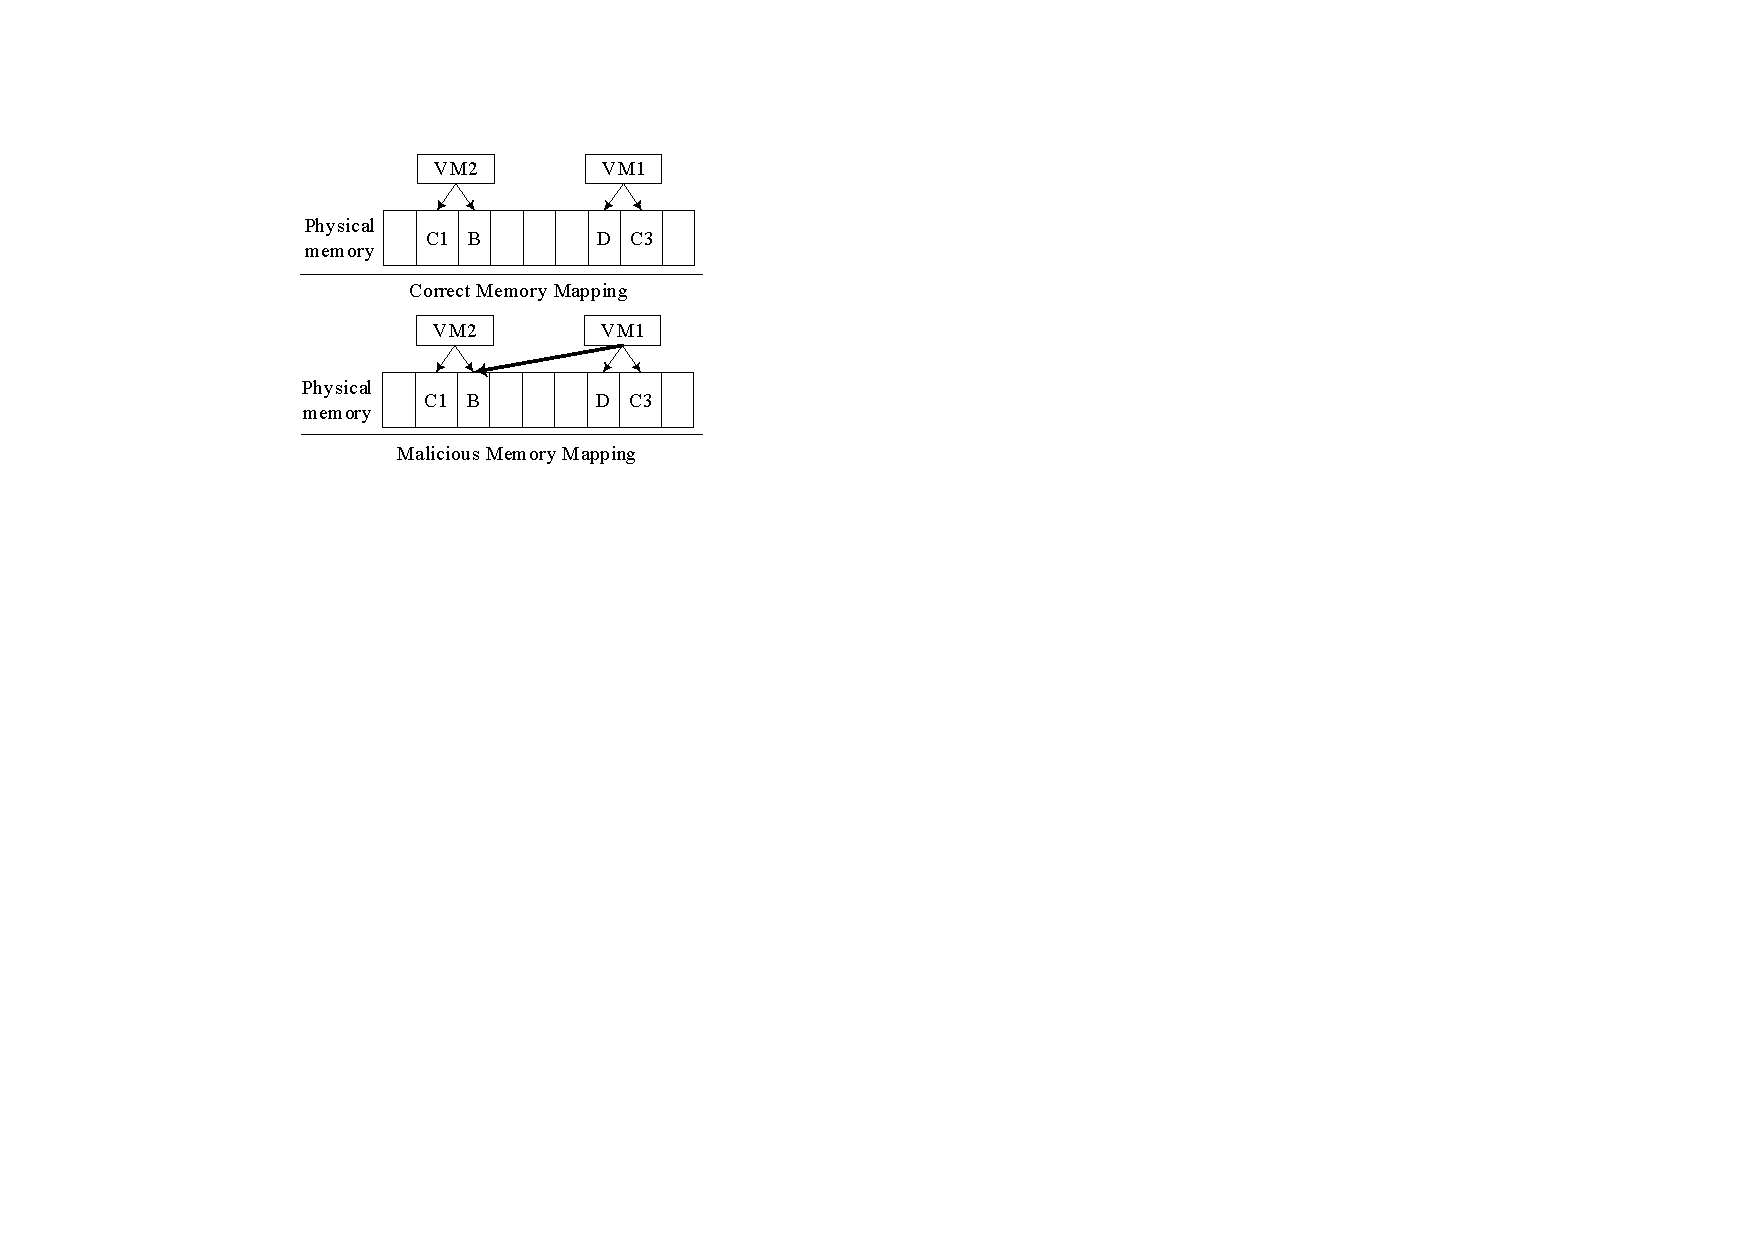
\includegraphics{IMG/remap.pdf}
    \caption{Diagram of Remapping Attack}
    \label{pic:remap}
\end{figure}

\subsubsection{Attacks to Kernel Page Tables}
We also take into account the fact that attacker already knows the deployment of HyperPS. As depicted in Figure \ref{pic:panorama}, key components, such as Kernel Page Tables, Control Registers, to create the secure and isolated execution environment are also protected by us. More details about the creation of the secure and isolated execution environment are illustrated in Section. 
%TODO 添加关于章节的引用
 
\subsection{Threat Model} \label{sub:threatmodel}
In this paper, 
We assume that the HostOS/Hypervisor has been compromised and controlled by the powerful adversary. The adversary can turn off kernel security mechanisms, such as DEP, SMEP, SMAP, and so on. The adversary can tamper fields of VMCSs and EPTs with dedicated malicious values. The adversary can also tamper VMCSs and EPTs through DMA write or regular memory access to them.  

We assume that the adversary does not possess the capability to conduct side channel attack and Hardware-based attack. We also assume that the adversary is unwilling to conduct the Denial of Service attack (DOS). In this paper, we assume that hardware resources are trusted, including processor, buses, BIOS/UEFI, and so on. 

%原威胁模型写的有问题。给出的两个例子后面写危害VMCS和
















